\section{Introduction}

\subsection{Order of an Ideal over PID ring}

PID -> every ideal is generated by one element, every module is an image of a free module, hence it can be expressed as $M\cong R/I_1\oplus...\oplus R/I_n$ for some ideals $I_i$. This allows as to define order of a module as $\ord(M)=\ord(I_1...I_n)$, which is the element that generates the ideal $I_1....I_n$. 

$\ord(M)$ can also be described using equivalence relation $M\sim M_1 + M_2\iff 0\to M_1\to M\to M_2\to 0$ is an exact sequence -> finitely generated abelian groups as $\Z$ modules and vector fields over $\mathfrak{K}$ as $\mathfrak{K}[x]$-modules.

\subsection{The Problem of non-PID rings}

Not every ring is a PID -> we must either find another invariant or make the ring in question a PID. E.g. for $\Z[x, x^{-1}]$ we can tensor it with some field, usually $\Q$ but we might want to try $F_p$ for some prime $p$.

Maybe some example for $\Z[x]$?

\subsection{Short Introduction to Knot Theory?}

Knot - a closed curve immersed in some $3$-dimensional space, or $S^1$ immersed in $S^3$

We will consider only tamed knots? That is knots that can be represented as a sum of a finite amount of straight lines?

Using Mayer-Vietoris sequence we can deduce that $H^1(S^3\setminus K)=\Z$ for any knot $K$. Hence, if we want to find interesting invariants, we must look further. 

Seifert surface of knot $K$ is an orientable surface whose boundary is $K$. We can use it to create an infinite cyclic covering of $S^3\setminus K$ by cutting copies $S^3\setminus K$ along this surface and gluing the $+$ side of Seifert surface of one copy to the $-$ side of the next copy.

$H^1(K^*)$ is more complicated than $H^1(S^3\setminus K)$ and things get interesting if we consider it as a $\Z[\Z]$ (or $\Z[x, x^{-1}]$-module. We can use the fact that $\Pi_1(K^*)^{ab}=H^1(K^*)$ and calculate this module to obtain something called Alexander ideal $I$: $H^1(K^*)\cong \Z[\Z]/I$. If $I$ is a principal ideal, e.g. in the case of trefoil knot of figure eight knot, its generator is called "Alexander polynomial". If this is not the case, we must consider $H^1(K^*; \Q)$ - kohomology module with coefficients in $\Q$, to obtain the Alexander polynomial. In the following paper we will consider what happens if we use $F_p$, a finite field, instead of $\Q$.

The matrix method

\subsection{Fast notes}

{\color{blue}
We might consider a module $M$ over some ring $R$, usually $R=\Z[t, t^{-1}]$. Let $K$ be a knot with $l$ arches and $s$ crossings that is oriented. We will consider a function $M^{l}\to M^{s}$ given by
$$+: au+bi+co = 0$$
$$-: \alpha u+\beta i + \gamma o = 0,$$
where $+$ or $-$ depends on what arches $u$, $i$ and $o$ create:
\begin{center}
  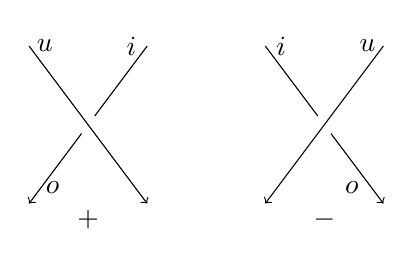
\begin{tikzpicture}
    \draw[<-] (0, -2)--(1.5, 0);
    \fill[white] (0.75, -1) circle (4pt);
    \draw[->] (0, 0)--(1.5, -2);

    \node at (0.75, -2.2) {$+$};
    \node at (0.2, 0) {$u$};
    \node at (1.3, 0) {$i$};
    \node at (0.3, -1.8) {$o$};

    \draw[->] (3, 0)--(4.5, -2);
    \fill[white] (3.75, -1) circle (4pt);
    \draw[<-] (3, -2)--(4.5, 0);
    
    \node at (3.75, -2.2) {$-$};
    \node at (3.2, 0) {$i$};
    \node at (4.3, 0) {$u$};
    \node at (4.1, -1.8) {$o$};
  \end{tikzpicture}
\end{center}
The kernel of this morphism is responsible for coloring of knot $K$. 

$a, b, c$ (and greek) are morphisms $M\to M$ (or $M\to N$ in more general case). We can assume that $c$ is a unit or even $c=1=\gamma$.

Furthermore, we can use equations above to obtain two operators $M\times M\to M\times M$ such that $(u,i)\mapsto (o, u)$ and $(i,u)\mapsto (u, o)$.

Two calculations on braids to do here, one that will give $a(a+b)=a$ and the other that states $ab=ba$ !! what is the difference when $a+b=1$ and when $a$ is not assumed to be a unit (therefore only $a^2+ab=a$)?

So now we can take a knot, its diagram and make it into a braid. A braid has a group (Burau representation, Markov knot theorem - moves) and we know that $\beta(w)v=v$ for the knot $w$ and any vector $v$.

the braid group $B_{n+1}$ with generators $\sigma_1, ..., \sigma_n$ can be send to $S_{n+1}$ with relation $\sigma\eta=\eta\sigma$ for translations that are disjoint and $\sigma\eta\sigma=\eta\sigma\eta$ ( i think ) but we might want to do something different and add a relation that sends $B_{n+1}$ to $H_{n+1}$ or however this algebra was named, using $\sigma^2+a\sigma+b=0$.

Going back to the $M\times M$ stuff -> we can have a matrix $\begin{bmatrix} 1-t & t\\ 1 & 0\end{bmatrix}$ and we can assosiate it with translation $\sigma_i$ from $B_{n+1}$ and it acts on the braid. This gives us a coloring of the braid.
}


\subsection{Coloring an unoriented knot diagram}

Let $R$ be a ring with identity and let $M$ be an $R$-module. If we consider a diagram of a knot $K$ without any orientation, the only type of crossing we will encounter is pictured in \cref{fig.1:unoriented:crossing}

\begin{figure}[h] \centering 
  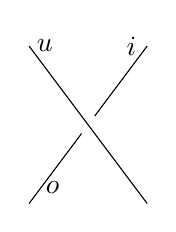
\begin{tikzpicture}
    \draw (0, -2)--(1.5, 0);
    \fill[white] (0.75, -1) circle (4pt);
    \draw (0, 0)--(1.5, -2);

    \node at (0.2, 0) {$u$};
    \node at (1.3, 0) {$i$};
    \node at (0.3, -1.8) {$o$};
  \end{tikzpicture}
  \caption{\label{fig.1:unoriented:crossing}Crossing in an unoriented knot diagram.}
\end{figure}

Notice, that rotating it by $180$ degrees changes $i$ and $o$ position (see \cref{fig.2:unoriented:crossing:floped}). Thus, segments passing under a crossing are indistinguishable. 

\begin{figure}[h] \centering 
  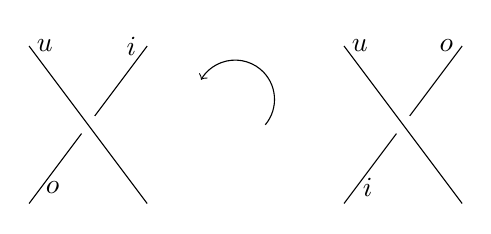
\begin{tikzpicture}
    \draw (0, -2)--(1.5, 0);
    \fill[white] (0.75, -1) circle (4pt);
    \draw (0, 0)--(1.5, -2);

    \node at (0.2, 0) {$u$};
    \node at (1.3, 0) {$i$};
    \node at (0.3, -1.8) {$o$};

    \draw[->] (3, -1) arc (-40:150:0.5);

    \draw (4, -2)--(5.5, 0);
    \fill[white] (4.75, -1) circle (4pt);
    \draw (4, 0)--(5.5, -2);

    \node at (4.2, 0) {$u$};
    \node at (5.3, 0) {$o$};
    \node at (4.3, -1.8) {$i$};
  \end{tikzpicture}
  \caption{\label{fig.2:unoriented:crossing:floped}Segments going under a crossing in an unoriented knot diagram are indistinguishable.}
\end{figure}

When $K$ has $s$ segments and $x$ crossings, we can write a labeling homomorphism
$$\phi:M^s\to M^x$$
which for segments that form a crossing pictured in \cref{fig.1:unoriented:crossing} takes value
$$\phi(u, i, o)=au+bi+co$$
for fixed $a,b,c\in\End(M)$. However, as we noted before, $i$ and $o$ are indistinguishable in \cref{fig.1:unoriented:crossing} and thus $b=c$, which yields a simpler definition:
%that assigns each element $m$ of $M^s$ an arbitrary value dependent on $a,b,c\in\End(M)$ are fixed endomorphisms and its relation to other segments. However, because $i$ and $o$ are impossible to tell apart, we must take $b=c$ and this arrive at a simpler function:
$$\phi(u,i,o)=au+b(i+o).$$

{\color{yellow}tutaj trzeba sie dokladnie zastanowic jak to idzie bardzo formalnie w zapisie
$${\color{red}\phi(u+i+o)=}au+bi+co=0$$
for $a, b, c\in \End(M)$ that are fixed for the entirety of $K$. However, because $i$ and $o$ are impossible to tell apart, we must take $b=c$ and thus arrive at a very simple equation:
%in fact have a very simple equation:
$$au+b(i+o)=0.$$
}

A coloring of a knot diagram without orientation is a labeling of its segments with elements from some module that agrees on crossings. That is, if a segment started in one crossing with label $x$ then it must be labeled with $x$ in every other crossing until another segment passes over it. Every diagram has a trivial coloring, in which every segment is labeled with the same element.

In other words, a coloring is an element from $M^s$ that agrees with $a$ and $b$ on every crossing and thus it belongs to $\ker\phi$. For $(m_1,...,m_s)\in\ker\phi$ we have a coloring such that segment $i$ is labeled with $m_i$.

{\color{yellow}If we extend the morphism $M^s\to M^x$ to an exact sequence, we obtain
$$0\to \ker\phi\to M^s\xrightarrow{\phi}M^x\to \coker\phi\to 0.$$
Module $\ker\phi$ can be viewed as a coloring of the diagram of $K$ with elements of module $M$.}

\begin{example}
  Let $M=\Z_n$, $R=\Z$, and consider the trefoil knot with $3$ segments and $3$ crossings.

  \begin{figure}[h] \centering
  \begin{tikzpicture}
    \begin{knot}[
      consider self intersections,
      flip crossing=2,
      clip width=20,
      ]
      \strand[thick]
      (90:2) to[out=180,in=-120,looseness=2]
      (-30:2) to[out=60,in=120,looseness=2]
      (210:2) to[out=-60,in=0,looseness=2] (90:2);
    \end{knot}
    \node at (130:2) {$l_1$};
    \node at (210:2.3) {$l_2$};
    \node at (-30:2.3) {$l_3$};
  \end{tikzpicture}

  \begin{tikzpicture}
  \fill (90:2.5) circle (2pt);
\fill (-30:3) circle (2pt);
\fill (210:3) circle (2pt);

\draw (90:2.5)
  \end{tikzpicture}
  \caption{An alternating diagram of trefoil knot $3_1$.}
\end{figure}

{\color{orange}TO DO: function such that $2x-y-z=0$ always when $x$ is the upper strand, using Smith's normal form show that only $\Z_3$ can be used to make a non-trivial coloring}

{\color{blue}MAYHAPSE A DIFFERENT KNOT?}

\end{example}

\subsection{The case of oriented knot diagram}



\begin{center}
  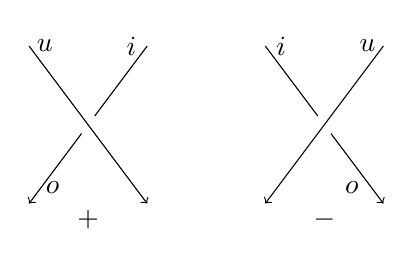
\begin{tikzpicture}
    \draw[<-] (0, -2)--(1.5, 0);
    \fill[white] (0.75, -1) circle (4pt);
    \draw[->] (0, 0)--(1.5, -2);

    \node at (0.75, -2.2) {$+$};
    \node at (0.2, 0) {$u$};
    \node at (1.3, 0) {$i$};
    \node at (0.3, -1.8) {$o$};

    \draw[->] (3, 0)--(4.5, -2);
    \fill[white] (3.75, -1) circle (4pt);
    \draw[<-] (3, -2)--(4.5, 0);
    
    \node at (3.75, -2.2) {$-$};
    \node at (3.2, 0) {$i$};
    \node at (4.3, 0) {$u$};
    \node at (4.1, -1.8) {$o$};
  \end{tikzpicture}
\end{center}



